\subsection{Zahlentheorie} \label{sec:zahlentheorie}
Auch wenn Fermat wichtige Beiträge zur Analysis und zur Stochastik geleistet hat, finden sich seine größten und bekanntesten Werke im Gebiet der \Gls{Zahlentheorie}. Dies war Fermats Lieblingsgebiet. Dabei spielt das Buch \textit{\say{Arithmetica}} von Diophantus eine wichtige Rolle, da es viele Ideen von Fermat im Gebiet der \Gls{Zahlentheorie} entfacht hat. Oft hat er Notizen oder neue Ideen an den Rand seiner Kopie von Arithmetica geschrieben. Die Bekanntesten seiner Ideen werden folgend vorgestellt. Wenn nicht anders beschrieben, dann sind alle Variablen grundsätzlich eine ganze Zahl ($\mathbb{Z}$).

Um die Kapitel \ref{sec:2sqr} und \ref{sec:faktorMethode} besser zu verstehen, muss das Konzept der \Gls{Kongruenz} in der \Gls{Zahlentheorie} erklärt werden.\footnote{Die Definition aller komplexen mathematischen Begriffe und Symbole sind, wie bereits erwähnt, im Glossar auf Seite \pageref{sec:glossary} und im Symbolverzeichnis auf Seite \pageref{sec:symb} zu finden.} Für die \Gls{Kongruenz} wird das Symbol \glssymbol{Kongruenz} verwendet. Grundlegend wird die Schreibweise \say{$a \equiv b \pmod{m}$} benutzt (sprich \say{$a$ und $b$ \glslink{Kongruenz}{kongruent} modulo $m$}), welche beschreibt, dass der Rest von $\frac{a}{m}$ und $\frac{b}{m}$ gleich ist. Als Beispiel kann lässt sich \say{$9 \equiv 17 \pmod{8}$} nehmen, da $9 : 8 = 1 \text{ Rest } 1$ und $17 : 8 = 2 \text{ Rest } 1$. Im Endeffekt ist es aber nichts anderes als $(a \bmod m) = (b \bmod m)$.

\subsubsection{Zwei-Quadrate-Satz} \label{sec:2sqr}
Fermat hat folgendes behauptet:

\begin{quote}
    Eine ungerade \Gls{Primzahl} kann als eine Summe von zwei \glslink{Quadratzahl}{Quadraten} $p = x^2 + y^2$ dargestellt werden, wobei $x$ und $y$ \glslink{Natuerliche Zahl}{natürlich} sind, wenn, und nur wenn $p \equiv 1 \pmod{4}$.
\end{quote}

Zur Einfachheit halber lässt sich die Bedingung \say{$p \equiv 1 \pmod{4}$} auch als \say{Wenn $p$ als $4n+1$ darstellbar ist} umformulieren. Schauen wir uns ein paar Beispiele an.

\begin{itemize}
    \item 17 ist \glslink{Primzahl}{prim} und kann als $4 \cdot 4 + 1$ dargestellt werden, daher ist der Zwei-Quadrate-Satz anwendbar: $17 = 4^2 + 1^2 = 16 + 1$
    \item 29 ist \glslink{Primzahl}{prim} und ist $4 \cdot 7 + 1$: $\quad 29 = 5^2 + 2^2 = 25 + 4$
    \item 37 ist \glslink{Primzahl}{prim} und ist $4 \cdot 8 + 1$: $\quad 37 = 6^6 + 1^2 = 36 + 1$
    \item 7 ist \glslink{Primzahl}{prim}, kann aber nicht als $4n + 1$ dargestellt werden, daher ist 7 auch nicht als eine Summe von zwei \glslink{Quadratzahl}{Quadraten} darstellbar.
\end{itemize}

Fermat hatte behauptet, den Zwei-Quadrate-Satz mit der \glslink{Unendlicher Abstieg}{Methode des unendlichen Abstiegs} bewiesen zu haben. Eine Erklärung der Methode ist im Glossar zu finden. Er hat aber,wie man es von ihm gewohnt war, keinen Beweis niedergeschrieben. Der erste Beweis kam von Leonhard Euler 1747, nachdem er mehrere Jahre damit verbracht hatte einen Beweis zu finden. Dieser hatte ebenfalls den \glslink{Unendlicher Abstieg}{unendlichen Abstieg} genutzt.
Mittlerweile existieren verschiedene Beweise, die auf verschiedenen Konzepten basieren, darunter ein Beweis welcher gaußsche Zahlen nutzt \cite{woodbury}, oder auch ein Beweis in einem einzigen Satz. \cite{zagier}

\subsubsection{Faktorisierungsmethode} \label{sec:faktorMethode}

\begin{figure}[htb]
    \centering
    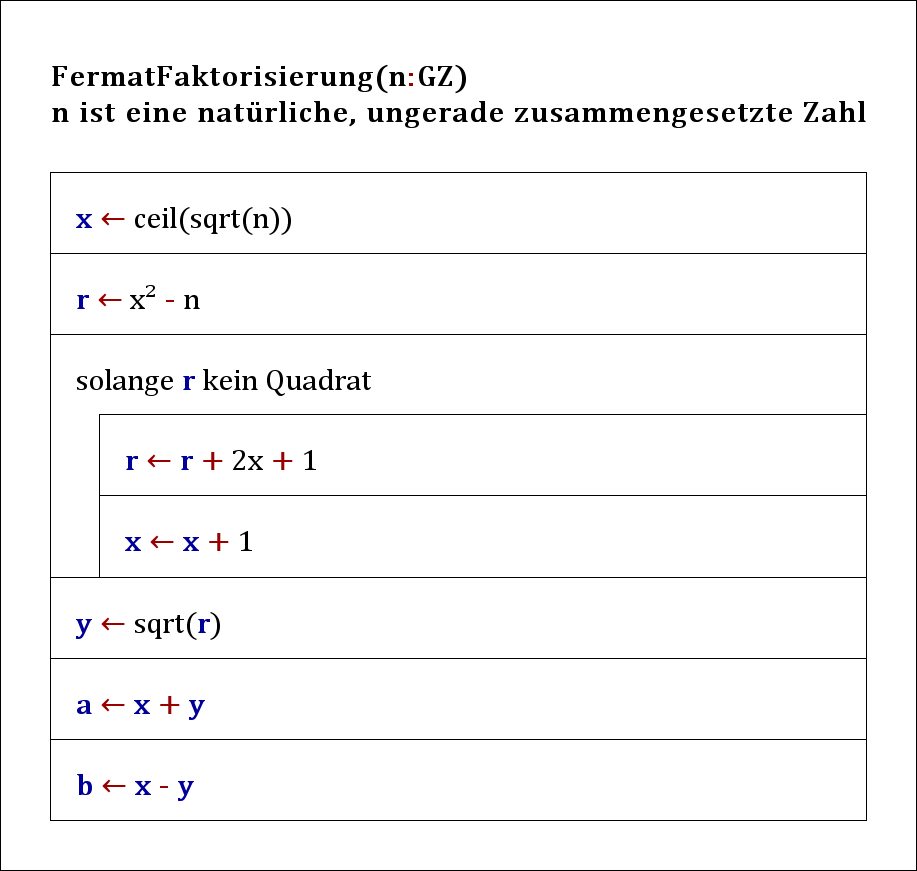
\includegraphics[width=0.75\textwidth]{img/factor_algorithm.png}
    \caption{Algorithmus von Fermats Faktorisierungsmethode in einem Struktogramm}
    \label{fig:factorAlgorithm}
\end{figure}

Die Faktorisierungsmethode von Fermat findet die \Glspl{Faktor} einer \glslink{Natuerliche Zahl}{natürlichen} ungeraden Zahl $n$, die aus mindestens zwei \Glspl{Primzahl} zusammengesetzt ist. Wenn die Faktorisierung von $n$ nun $n = a \cdot b$ ist, dann ist der Algorithmus für die Faktorisierungsmethode wie in Abbildung \ref{fig:factorAlgorithm} beschrieben. Dabei ist folgender Fakt grundlegend für die Faktorisierung:

\begin{theorem}
    Jede ungerade Zahl kann als eine Differenz von zwei \glslink{Quadratzahl}{Quadraten} dargestellt werden.
\end{theorem}
\begin{proof}
    Wenn man nun annimmt, dass sich eine ungerade Zahl $n$ auch als \begin{equation} \label{eq:faktor2square}
        n = x^2 - y^2
    \end{equation}
    schreiben lässt, ist es möglich mit der dritten binomischen Formel die Gleichung zu
    \begin{equation} \label{eq:binom}
        n = (x+y)(x-y)
    \end{equation}
    umzuschreiben. Nun setzt man eine Variable $a$ und $b$ gleich der beiden Faktoren aus \eqref{eq:binom}, sodass $a = x + y$ und $b = x - y$. Wenn man nun auf $x$ und $y$ auflöst, dann bekommt man $x = \frac{a+b}{2}$ und $y = \frac{a-b}{2}$. Eingesetzt in \eqref{eq:faktor2square} ergibt es

    \begin{align*}
        n & = \left( \frac{a+b}{2} \right)^2 - \left( \frac{a-b}{2} \right)^2 \\
          & = \dfrac{a^2 + 2ab + b^2 - a^2 + 2ab - b^2}{4}                    \\
          & = \dfrac{4ab}{4} = ab
    \end{align*}

    Somit kann jede ungerade Zahl kann als eine Differenz von zwei \glslink{Quadratzahl}{Quadraten} dargestellt werden.

\end{proof}

Dies wird nun genutzt, es wird solange eine Zahl $y$ gesucht, bis diese eine \Gls{Quadratzahl} ist. Da jede ungerade Zahl als Differenz von zwei \glslink{Quadratzahl}{Quadraten} dargestellt werden kann und eine dann bereits gefunden wurde, lässt sich die andere leicht durch Subtraktion finden. Nun hat man zwei Faktoren $a$ und $b$ von $n$ gefunden. Da $n$ ungerade ist, müssen die beiden Faktoren auch ungerade sein, da $n$ sonst gerade wäre. Wenn $a$ oder $b$ noch keine Primzahlen sind, dann kann man die gleiche Methode nutzen, um für jeweils $a$ oder $b$ die Faktoren zu finden. So hat Fermat bereits 1643 eine Primfaktorzerlegung von der Zahl $2.027.651.281$ durchgeführt. Auch dieser Beweis wurde von Fermat mit ins Grab genommen.

\subsubsection{Kleiner Satz} \label{sec:klSatz}
Fermats kleiner Satz ist der zweitbekannteste von Fermats Werken, nach dem großen Satz, er wird \say{klein} genannt, um ihn nicht mit dem Großen zu verwechseln. Dieser wurde 1640 in einem Brief von Fermat zu Bernard Frénicle de Bessy vorgestellt. Fermat hat den Satz als folgende Aussage vorgestellt:

\begin{quote}
    Wenn $p$ \glslink{Primzahl}{prim} und $a \nmid p$ ($a$ nicht durch $p$ teilbar), dann gilt
    \begin{equation} \label{eq:klSatz1}
        a^{p-1} \equiv 1 \pmod{p}
    \end{equation}
\end{quote}

\noindent Dies kann man auch als

\begin{quote}
    Wenn $p$ \glslink{Primzahl}{prim} und $a$ ganzzahlig, dann gilt
    \begin{equation} \label{eq:klSatz2}
        a^p \equiv a \pmod{p}
    \end{equation}
    sodass $a^p - a$ ein Mehrfaches von $p$ sein muss.
\end{quote}

\noindent formulieren, auch wenn die Anfangsbedingungen offener aussehen. Dies ist möglich, da die Formel \ref{eq:klSatz1} voraussetzt, dass $a \nmid p$. Daher muss es auch eine Zahl $b$ geben, sodass $ab \equiv 1 \pmod{p}$, da $a$ ansonsten keinen Teiler hätte. Wenn also nun $a^p \equiv a \pmod{p}$ und beide Seiten mit $b$ multipliziert werden, lässt sich auf beiden Seiten ein $a$ herauskürzen und es kommt $a^{p-1} \equiv 1 \pmod{p}$ heraus, welches somit äquivalent zu Formel \ref{eq:klSatz2} ist. Ein paar Beispiele:

\begin{itemize}
    \item Wenn $a=2$ und $p=5$, dann $2^{5} = 32 = 2 \cdot 16$. Damit lässt sich $2^{5}$ als ein Mehrfaches von 2 darstellen.
    \item Wenn $a=5$ und $p=13$, dann $5^{13} = 1220703125 = 5 \cdot 244140625$.
    \item $a=35$ und $p=19$: \quad $35^{19} = 217416671473944530487060546875 \\ = 35 \cdot 6211904899255558013916015625$
\end{itemize}

Mittlerweile gibt es einige Methoden um den Satz zu beweisen. Anders als der Beweis des großen Satzes von Fermat, passt der des kleinen Satzes leicht auf die Rückseite einer Postkarte. Da alle aber für den durchschnittlichen Leser etwas schwerer zu verstehen sind, werde ich darauf verzichten einen zu umfassen. Ein Beweis mit dem binomischen Lehrsatz lässt sich in \cite{wolframFlT} finden. Der Beweis von Fermat selber ist, wie man es sich schon denken kann, nirgendwo zu finden.

Auf dem kleinen Satz aufbauend ist der Satz von Euler, welcher eine Verallgemeinerung des kleinen Satzes darstellt, wobei $p$ nicht \glslink{Primzahl}{prim} sein muss. Der kleine Satz wird heutzutage als Basis für den fermatschen Primzahltest und in der heutigen Kryptografie als Basis der RSA-Verschlüsselung genutzt.

\subsubsection{Großer Satz} \label{sec:grSatz}
Der große Satz von Fermat, auch \say{Fermats letzter Satz} oder \say{Fermatsche Vermutung} genannt, ist sein bekanntestes Problem. Der Name \say{Fermats letzter Satz} kommt nicht daher, dass es wortwörtlich der letzte Satz war den er aufgestellt hatte, sondern weil es der Satz von Fermat war, der als letztes bewiesen wurde. Den großen Satz bzw. die Problemstellung, sowie den Beweis, hat er selbst nie veröffentlicht. Erst fünf Jahre nach seinem Tod hat einer seiner Söhne die zahlreichen Randnotizen in Fermats Kopie von Diophantus \say{Arithmetica} gefunden und veröffentlicht. Aufgestellt in ca. 1637 findet sich folgende Notiz am Rande:

\begin{quote}
    \textit{\say{Es ist unmöglich eine Zahl dritter Potenz in zwei Zahlen dritter Potenzen, oder eine Zahl vierter Potenz in zwei Zahlen vierter Potenzen, oder allgemein, jede Potenz höher als 2 in die zwei gleichen zu zerlegen. Ich habe einen wahrlich wunderbaren Beweis für dieses Problem entdeckt, für den dieser Buchrand zu eng ist.}}
    \footnote{Cubum autem in duos cubos, aut quadratoquadratum in duos quadratoquadratos \& generaliter nullam in infinitum ultra quadratum potestatem in duos eiusdem nominis fas est dividere cuius rei demonstrationem mirabilem sane detexi. Hanc marginis exiguitas non caperet.}
\end{quote}

Allgemein formuliert bedeutet das:
\begin{quote}
    Die Gleichung $x^n + y^n = z^n$ mit $n,x,y,z \in \mathbb{N}$ hat für $n>2$ keine ganzzahlige Lösung.
\end{quote}

Dass es für $n = 2$ unendlich viele Lösungen gibt, wussten schon die Griechen. Man muss nur das Stichwort \say{Satz des Pythagoras} sagen und es sollte einem direkt die Zahlengruppe $3,4,5$ einfallen, welche für $n = 2$ die gültige Lösung $3^2 + 4^2 = 5^2$ bildet. Zwar hat Fermat nicht den gesamten Satz bewiesen, dafür aber den Fall $n = 4$ mit seiner eigen entwickelten Methode des \glslink{Unendlicher Abstieg}{unendlichen Abstiegs}, dessen Beschreibung im Glossar zu finden ist.

Einfach zu verstehen wie er war, haben viele Mathematiker versucht den großen Satz von Fermat zu beweisen, jedoch sind alle am Versuch gescheitert. Über mehrere Jahrhunderte blieb die Lösung ein Mysterium. Erst 350 Jahre später hat Andrew Wiles 1995 einen kompletten Beweis des großen Satz von Fermat veröffentlicht. Dieser war schon seit seiner Kindheit, als er zehn Jahre alt war, von der Einfachheit des großen Satzes fasziniert und hat sich seitdem vorgenommen, diesen als Erstes zu beweisen. Da er aber schnell gemerkt hatte, dass es mit seinem mathematischen Wissen zu dieser Zeit nichts werden könne, hat er, erst nachdem er 33 geworden war, die Suche fortgesetzt. Nach mehr als 6 Jahren geheimgehaltener und akribischer Forschung hatte er 1993 den Beweis vorgetragen, mit dem Titel \say{Modular Forms, Elliptic Curves and Galois Representations.}. Dieser hatte sich nicht anmerken lassen, dass es sich hierbei um den Beweis Fermats großen Satz handelt. Erst am Ende des dritten und letzten Vortrags hat er nebenbei angemerkt, dass er nun den Satz bewiesen hatte. \cite{newYorkTimes} Im August wurde aber ein Fehler im Beweis entdeckt, den Wiles erst in September 1994 korrigieren konnte und Mai 1995 dann neu veröffentlicht hat. Für den Beweis hat er viele Preise und Auszeichnungen erhalten und er gilt als eines der wichtigsten Fortschritte der modernen Mathematik.

Den großen Satz hier zu beweisen würden den kompletten Rahmen der Arbeit sprengen. Wer einen Blick in Wiles 109 Seiten langen Beweis werfen möchte, findet diesen in \cite{wilesFermat}. Der Beweis behandelt den Modularitätssatz (früher auch \say{Taniyama-Shimura-Vermutung} genannt) und elliptische Kurven. Wiles beweist den schwierigsten Teil davon, welches gleichzeitig den großen Satz impliziert. Der vollständige Beweis des Modularitätssatzes ist 2001 gefunden worden. Ein Buch, welches den großen Satz und damit auch den Modularitätssatz weiter im Detail behandelt findet sich hier \cite{darmon}.

Der Beweis des großen Satzes wurde erst nach 6 Jahren Forschungen mit mathematischen Mitteln des 20. Jahrhunderts gefunden, daher ist man sich heutzutage einig, dass Fermat zwar behauptet hat einen Beweis gefunden zu haben, aber doch nie einen hatte oder dass sein Beweis fehlerhaft war.
